\documentclass[a4paper]{ctexart}
\usepackage{lmodern}
\usepackage{amsmath}
\usepackage{amsthm}
\usepackage{graphicx}
\usepackage{enumerate}
\usepackage{listings}
\usepackage{xcolor}
\usepackage[textwidth=14.5cm]{geometry}
\usepackage{blindtext}
\parindent=0pt

% 设置文档中插入代码的显示格式:
\definecolor{mygreen}{rgb}{0,0.6,0}
\definecolor{mygray}{rgb}{0.5,0.5,0.5}
\definecolor{mymauve}{rgb}{0.58,0,0.82}
\lstset
{
  backgroundcolor=\color{white},   % choose the background color; you must add \usepackage{color} or \usepackage{xcolor}
  basicstyle=\footnotesize,        % the size of the fonts that are used for the code
  breakatwhitespace=false,         % sets if automatic breaks should only happen at whitespace
  breaklines=true,                 % sets automatic line breaking
  captionpos=bl,                   % sets the caption-position to bottom
  commentstyle=\color{mygreen},    % comment style
  deletekeywords={...},            % if you want to delete keywords from the given language
  escapeinside={\%*}{*)},          % if you want to add LaTeX within your code
  extendedchars=true,              % lets you use non-ASCII characters; for 8-bits encodings only, does not work with UTF-8
  frame=single,                    % adds a frame around the code
  keepspaces=true,                 % keeps spaces in text, useful for keeping indentation of code (possibly needs columns=flexible)
  keywordstyle=\color{blue},       % keyword style
  language=C++,                    % the language of the code
  morekeywords={*,...},            % if you want to add more keywords to the set
  numbers=left,                    % where to put the line-numbers; possible values are (none, left, right)
  numbersep=5pt,                   % how far the line-numbers are from the code
  numberstyle=\tiny\color{mygray}, % the style that is used for the line-numbers
  rulecolor=\color{black},         % if not set, the frame-color may be changed on line-breaks within not-black text (e.g. comments (green here))
  showspaces=false,                % show spaces everywhere adding particular underscores; it overrides 'showstringspaces'
  showstringspaces=false,          % underline spaces within strings only
  showtabs=false,                  % show tabs within strings adding particular underscores
  stepnumber=1,                    % the step between two line-numbers. If it's 1, each line will be numbered
  stringstyle=\color{orange},      % string literal style
  tabsize=2,                       % sets default tabsize to 2 spaces
  title=tile.cpp                   % show the filename of files included with \lstinputlisting; also try caption instead of title
}
\title{算法分析与设计 - 选做1}
\author{}
\date{2022/09/05}

\begin{document}
\begin{sloppypar}  % 控制页边距,防止行溢出

    % 标题:
    \maketitle

    % 第一章:
    \section{铺砖定理以及实现}
    \vspace{1em}  % 空一行

    % 定理:
    \newtheorem{theorem}{\bf 定理}
    \begin{theorem}[铺砖定理]
        在一个大小为$m * m$(m为2的幂)
        的正方形场地中(图~\ref{floor}),
        铺设形状如图~\ref{brick}所示的地砖,
        并且要在指定位置留出空缺(图~\ref{floor}中灰色部分),
        此类问题总是有解的.
        % 插入图片:
        \begin{figure}[h]
            \centering
            \begin{minipage}[t]{0.5\linewidth}
                \centering
                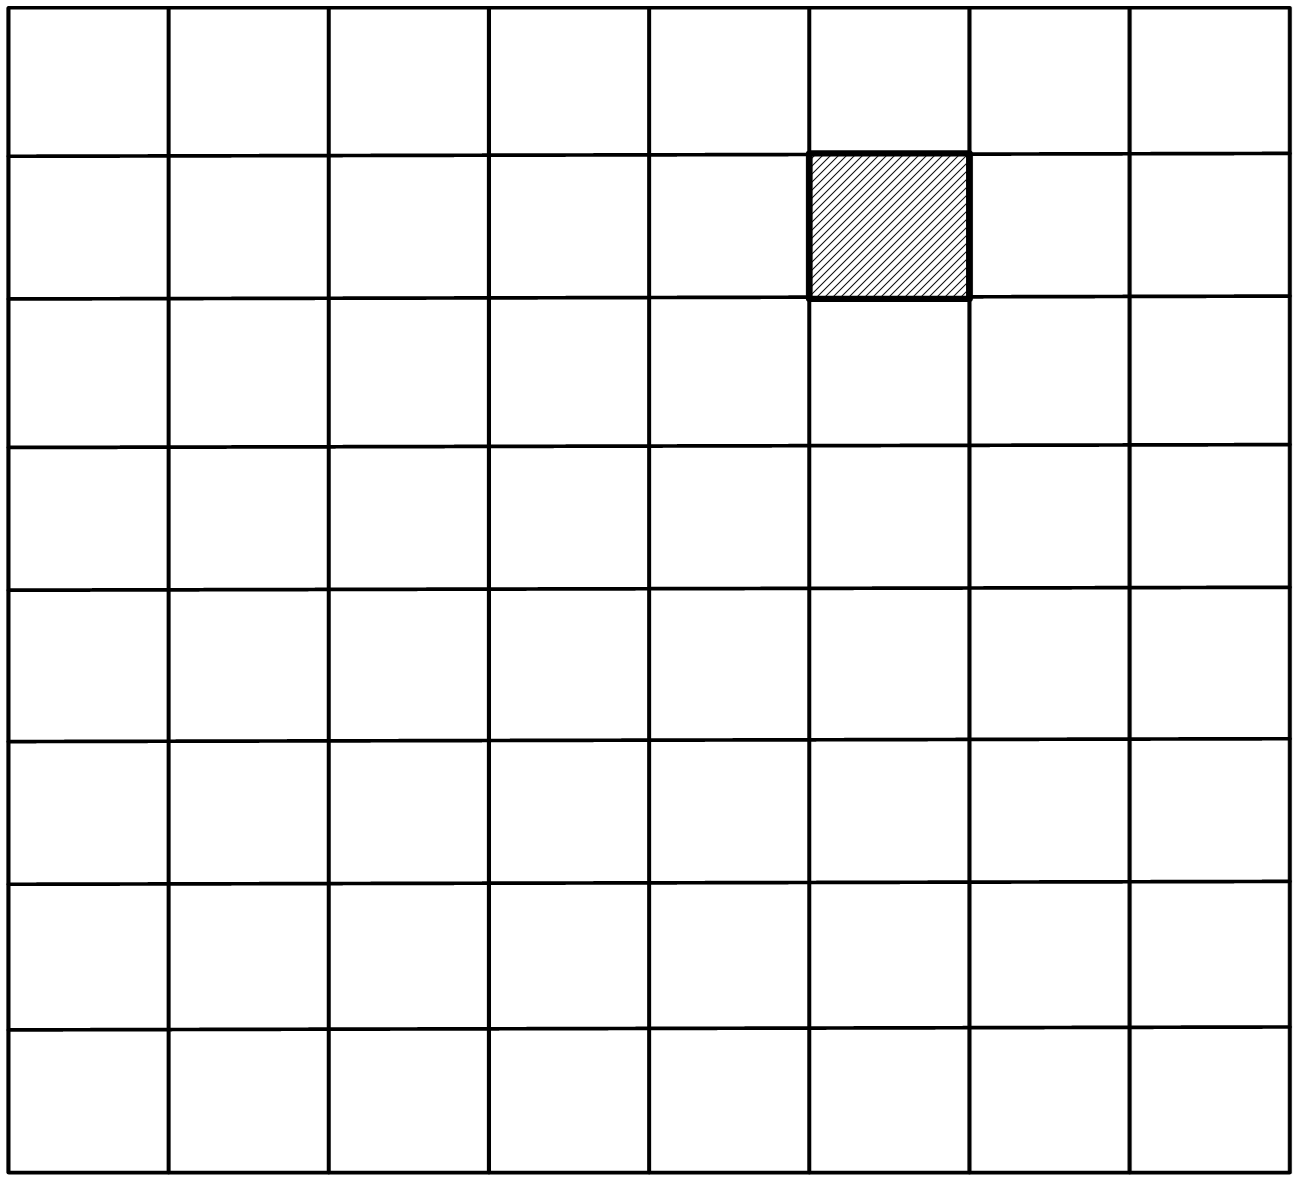
\includegraphics[scale=0.4]{images/floor.png}
                \caption{场地}
                \label{floor}
            \end{minipage}
            %\qquad
            \begin{minipage}[t]{0.3\linewidth}
                \centering
                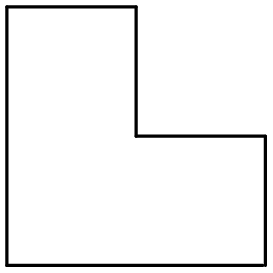
\includegraphics[scale=0.5]{images/brick.png}
                \caption{地砖}
                \label{brick}
            \end{minipage}
        \end{figure}
    \end{theorem}

    % 证明:
    \begin{proof}
        不妨设$m = 2^n$.
        \begin{enumerate}[1)]
            \item 当$n = 0$, 即$m = 1$时, 显然成立;
                  当$n = 1$, 即$m = 2$时, 有如图~\ref{4Cases}所示四种情况, 同样成立.
                  % 插入图片:
                  \begin{figure}[h]
                      \centering
                      
\includegraphics[scale=0.5]{images/4Cases.png}
                      \caption{$n = 1$时的四种情况}
                      \label{4Cases}
                  \end{figure}
            \item $\forall n \geq 1, m = 2^n$,
                  对$2^{n-1} * 2^{n-1}$大小的地板显然成立,
                  现四分地板得到4个相同大小的地板,
                  按照图~\ref{split}所示, 在边界位置铺砖,
                  使空缺所在地板之外的3块地板也变为存在空缺的地板,
                  之后递归进行填充, m不断缩小为原来的一半,
                  直到$m \leq 2$.
                  \qedhere  % 证毕符号
                  % 插入图片:
                  \begin{figure}[h]
                      \centering
                      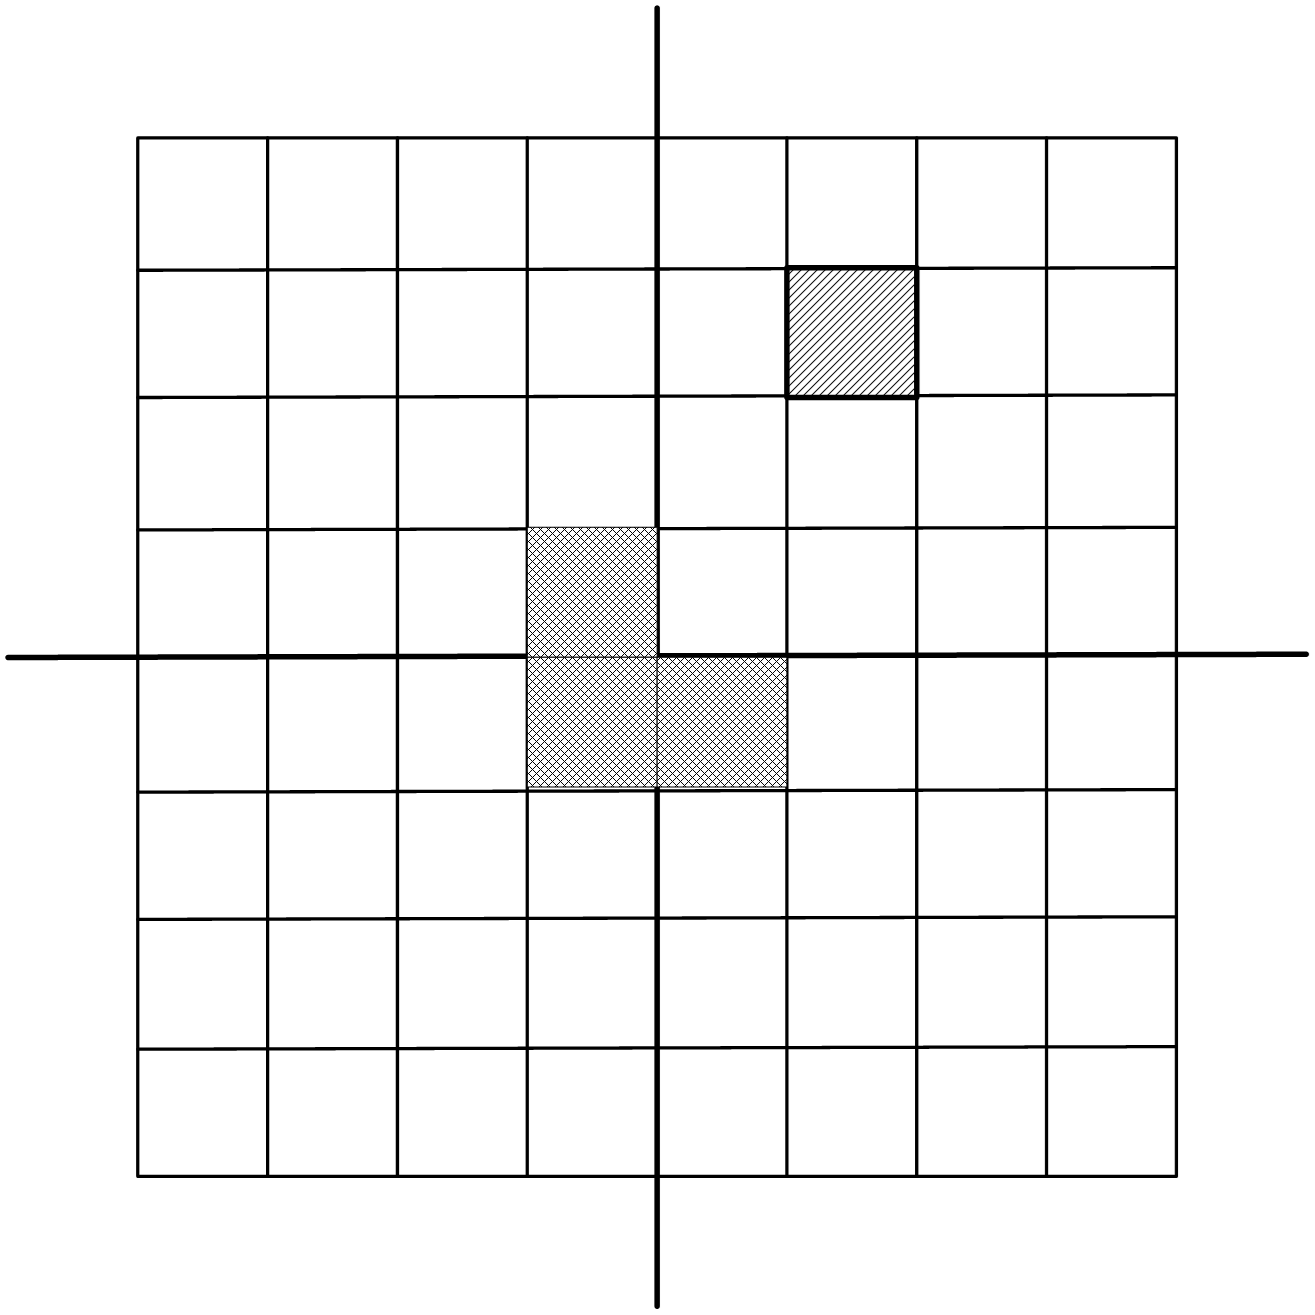
\includegraphics[scale=0.4]{images/split.png}
                      \caption{将地板划分为4块}
                      \label{split}
                  \end{figure}
        \end{enumerate}
    \end{proof}
    \vspace{1em}

    代码实现:\\
    (注释中有部分特殊符号因为字体原因不能正常显示)
    % 从文件插入代码:
    \lstinputlisting[language=C++, title=tile.c]{tile.cpp}
    \vspace{1em}

    运行结果:
    % 插入图片:
    \begin{figure}[h]
        \centering
        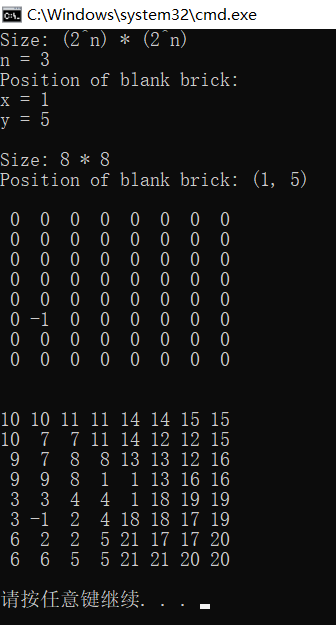
\includegraphics[scale=0.9]{images/test1.png}
        \caption{$n = 3, (x, y) = (1, 5)$}
    \end{figure}
    \begin{figure}[h]
        \centering
        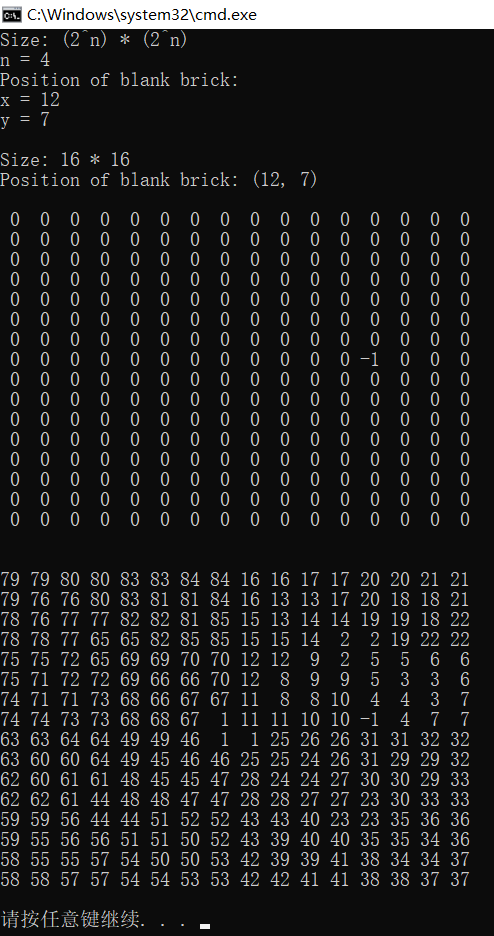
\includegraphics[scale=0.7]{images/test2.png}
        \caption{$n = 3, (x, y) = (12, 7)$}
    \end{figure}
\end{sloppypar}
\end{document}
